\section*{Introduction}

Seaborne measurements are often expensive and time consuming, though they can have a large impact on the area, where the data have been obtained. In 2011 the naval safe zone around the Fukusima accident was laid down based only on estimates of the radiation contamination\ref{res:FNPP}, because low amount of measurement data was avaialble due to high measurement costs and relatively low neccessity. Another area, the coastal waters of Greenland is very poorly mapped up to present day. Ships have to sail in a roundabout way around the island, because the risk of wrecking in unknows fjordic area is very high. This is a huge waste of time and natural resources annually.

Oceanographic measurements today are carried out by large crewed ships, but they could be replaced by a number of smaller crafts in order to reduce surveying time and cost, and increase the available manpower in other tasks. These vessels have the advantage of sailing previously unsurveyable areas as well, thanks to the shallower draught and smaller size.

The aim of this project is to develop an autonomus surface vehicle, which is capable of conducting arbitrary seaborne measurements. To execute an oceanography mission, the ship must be capable of autonomus navigation based on Global Positioning System (GPS) and an Internal Measurement Unit (IMU), to further enhance the precision in hazardous environment.

\begin{figure}[H]
	\centering
	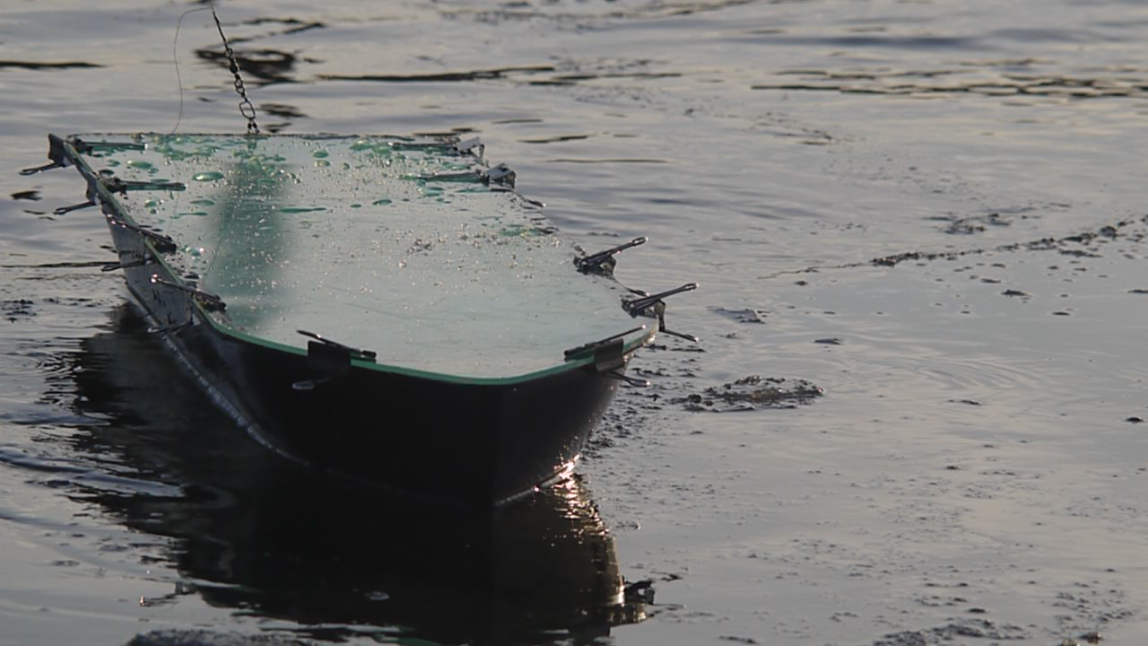
\includegraphics[width=0.8\textwidth]{img/aauship}
	\caption{The AAUSHIP prototype on her maiden voyage}
	\label{fig:aauship}
\end{figure}

\subsection*{Development guidelines}
In order to keep a sensible and extendable system, the control software of the ship follows the guidelines of the Model-Based Design approach. The system software can be divided to two different kind of modules, one that is dependent, and one that is independent from the physical characteristics of the vessel. In order to maximize the extendability of the system, the fix (independent) modules must be complelely general, but as thorough as possible, so as to keep the complexity of the changeable (dependent) software of the robot minimal.
\begin{wrapfigure}{r}{0.48\textwidth}
  \begin{center}
    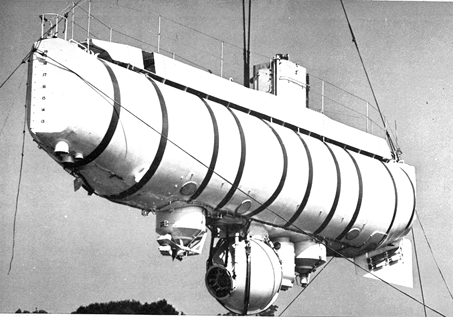
\includegraphics[width=0.5\textwidth]{img/trieste}
  \end{center}
  \caption{Bathyscaphe Trieste, the first manned vessel that reached the bottom of Challenger Deep (Mariana Trench)\cite{trieste}}
\end{wrapfigure}

The environment stored in the control system must be extendable to the third dimension, and must be able to track changes over time.
The tasks of the low level control must be as specific and as basic as possible. All calculations and control should be implemented in the high level controller.
the high level controller must be parametrized, based on the low level and hardware characteristics.

The point of these guidelines is to create a system of components with major reusability. Ideally a general Cross-platform High Level Controller controls different kind of vessels, through a standard interface. When changing to an arbitrary different vehicle, only the Low Level Controller must be replaced, which stores the characteristics of the vessel and implements the actuator control.

\subsection{Operation models}

 A typical oceanography application starts on the shore. A science team analyzes the currently available data, then marks the area of measurements on the map. The  map data is transformed to a measurement path by the scientists or by the automatic waypoint planner of the ship. The autonomus surface vehicle is then outfitted with the right sensors for the task, and a manned ship transports it close to its destination. The crew can set the research vessel to manual, automatic or fully autonomus mode.

\paragraph{Manual control}
In this mode it's possible for the operator to control the movement of the ship, degree of freedom-wise or control the actuators themselves. The primary intent of this mode is for testing or malfunction-recovery.

\begin{figure}[H]
	\centering
	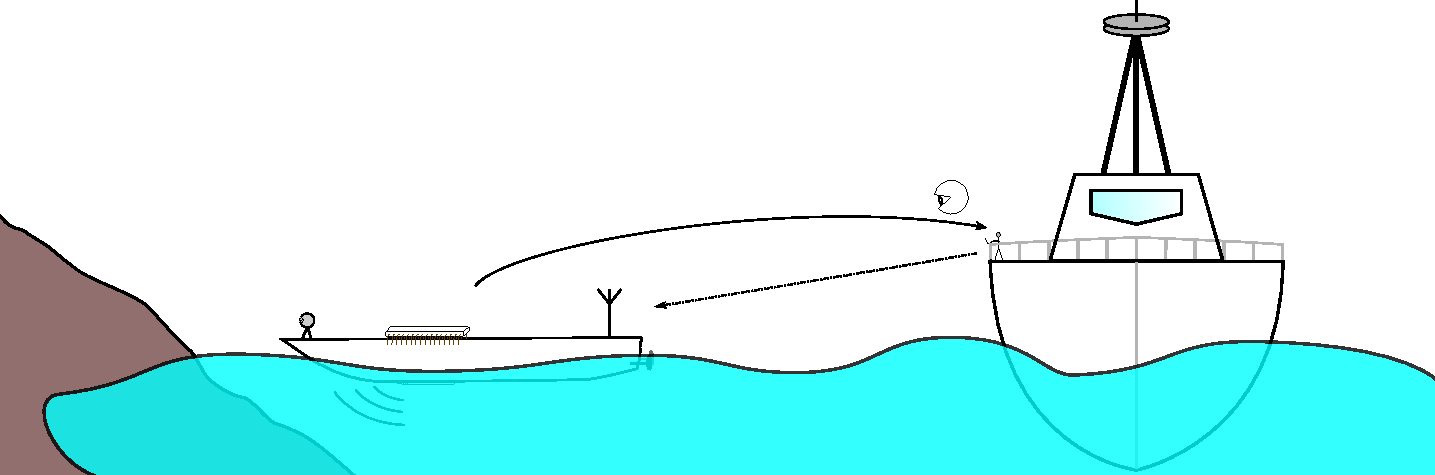
\includegraphics[width=0.8\textwidth]{img/manualcontrol}
	\caption{Manual remote control}
	\label{fig:manualcontrol}
\end{figure}

\paragraph{Automatic control}
In automatic mode the "brains", remain on the crewed vessel, and the research craft remains in wireless connection with the Mothership. When the measurements are complete, the oceanographer returns to the mothership. In automatic mode it is always possible to switch to manual control and back, or update the measurement path, etc.

\begin{figure}[H]
	\centering
	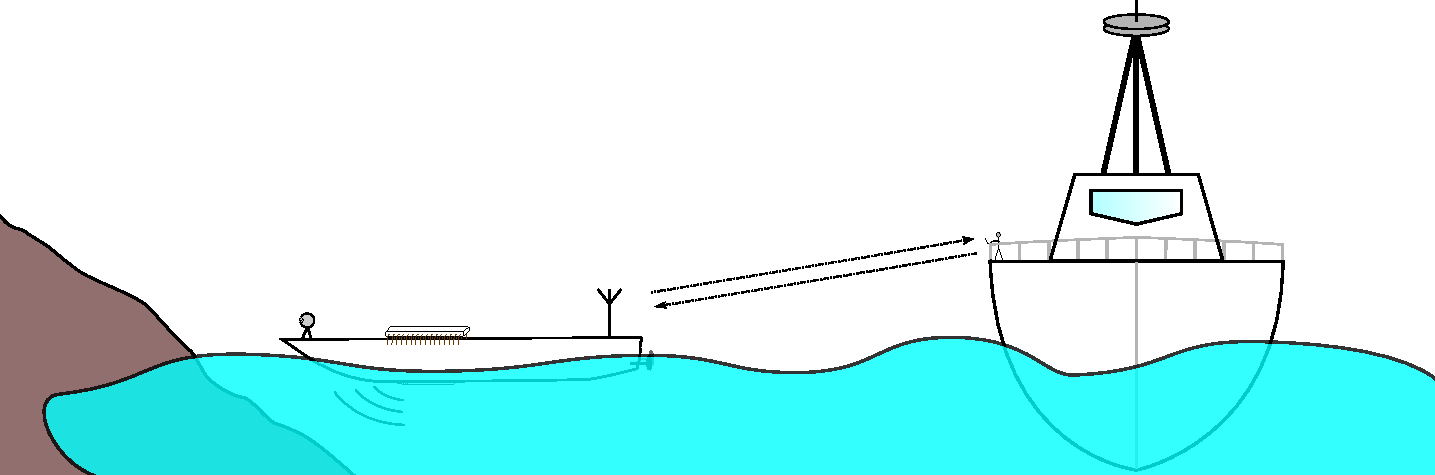
\includegraphics[width=0.8\textwidth]{img/automatic}
	\caption{Automatic supervised control}
	\label{fig:automatic}
\end{figure}

\paragraph{Autonomus control}
In Autonomus mode the ship carries everything that is needed to complete the task. Connection to the mothership can be cut, and the vessel carries the orders out autonomusly. Intervention in this mode is only possible until the oceanographer is in range of the mothership.

\begin{figure}[H]
	\centering
	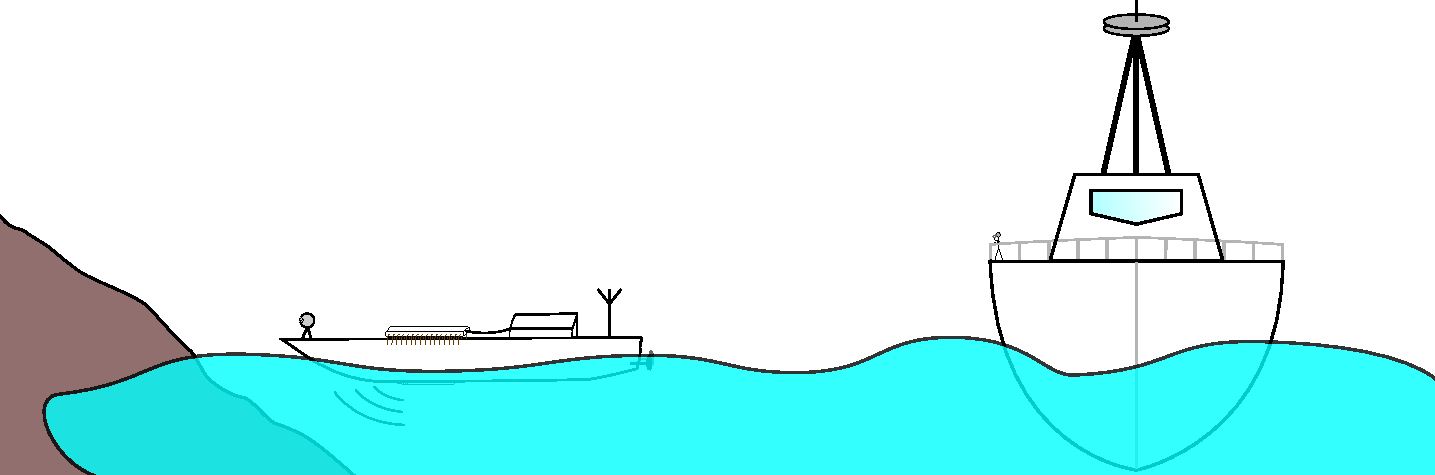
\includegraphics[width=0.8\textwidth]{img/autonomus}
	\caption{Autonomus control}
	\label{fig:autonomus}
\end{figure}

\paragraph{}
In case there are multiple research vessels, they can form a squadron. In this setup only one of the ships needs to be in range of the crewed mothership. Alternatively one autonomus ship is capable of controlling multiple automatic crafts, taking over the role of the mothership.

\begin{figure}[H]
	\centering
	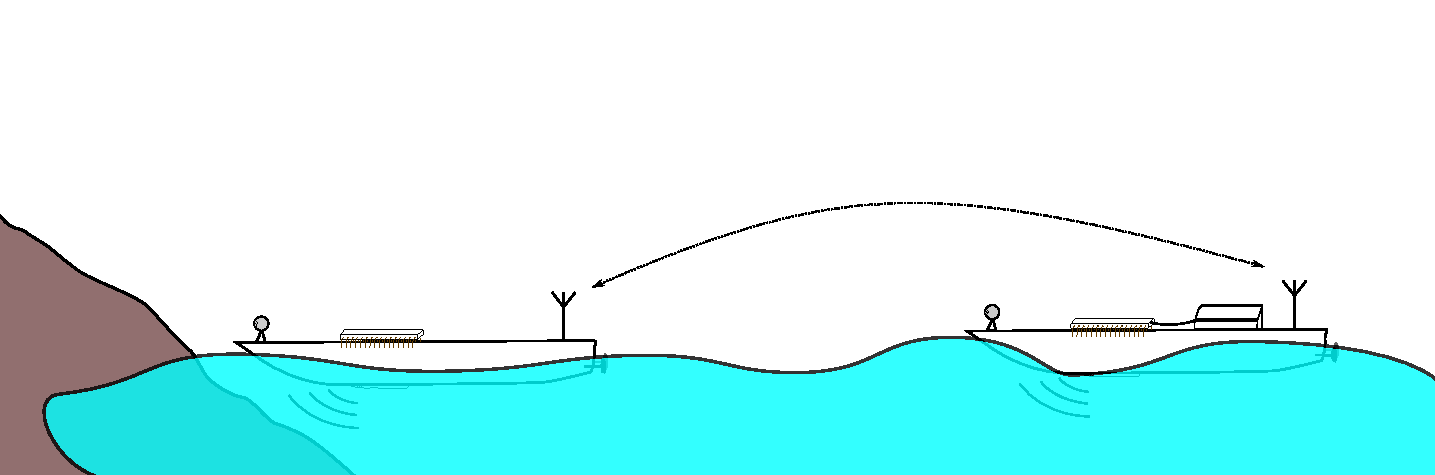
\includegraphics[width=0.8\textwidth]{img/multiple}
	\caption{Squadron mode}
	\label{fig:multiple}
\end{figure}

\begin{tcolorbox}[colback=cyan!5,colframe=cyan!40!black,title=Code: Main.py \\ https://www.dropbox.com/s/h1067ywmdajkegk/Main.py]
\begin{minipage}{0,6\textwidth}
The mission planning steps are implemented in Main.py, which is the main part of the program, responsible for initializing the system, setting the target area, mode of routing, navigation, etc. Later Main.py will provide a Graphical User Interface as well.
\end{minipage}
\begin{minipage}{0,35\textwidth}
\raggedleft

\includegraphics[width=0.8\textwidth]{img/main}
\end{minipage}

\end{tcolorbox}

In order to execute a rational oceanography task, a number of valid objectives must be set. These objectives are usually one or more of the following\cite{oceanography}:

\begin{itemize}
\item A set of geographical measurement locations, with or without time and measurement type conditions
\item A certain area that contains points of interest
\item Maximal action duration requirement
\item Other
\end{itemize}

The task planning is usually carried out by the scientist group, but some auto-planning modes need to be supported. A typical task is the creation of a measurement-grid, with preset definition, in a certain geographical area. The High Level Controller (HLC) uses a Mission planning time algorithm, to support the auto-generation of the waypoints. This module is the "Waypoint planner", which outputs a list of coordinates that contains the measurement points.

Once the ship reaches the current waypoint, it determines the next aim.

A set of points defining a path can be specified for the ship, but it does not ensure that the created path is valid, therefore a second "Pathplanning" stage is required, which analyzes the generated set of locations and creates a path that is actually sailable by the ship.
